	\begin{homeworkProblem}[Méthode statistique]
	
			Une approche souvent utilisée revient à filtrer les messages électroniques sur la base de
			leur contenu (content-based filtering). Un exemple classique consiste à filtrer les
			messages en fonction de la fréquence d’apparition de certains mots. Utilisez le fichier
			spambase afin d’appliquer une méthode statistique qui vous permettra de classifier les
			messages en deux catégories, soit spam (1) ou non spam (0).
			Compte tenu de la nature binomiale (0/1) de la variable dépendante, la régression
			logistique  peut être utilisée comme méthode de classification. Votre variable
			dépendante (0/1) représente la catégorie associée (spam ou non spam) et les variables
			indépendantes représentent la fréquence d’apparition de certains mots.	
	
		\begin{homeworkSection}{2.1}

			Effectuez une régression logistique en utilisant l’ensemble des variables (57)
			contenues dans le fichier spambase. Divisez les données afin d’en utiliser 66\% pour la
			phase d’apprentissage de votre modèle. À quoi servira l’autre 33\% ?
			Donnez pour chaque variable indépendante son coefficient ainsi que son « odd ratio »
			associé. Quelle est la signification de ces deux valeurs?\\

			\problemAnswer{
			
			Les premiers 66\% servent à établir notre modèle, et les derniers 33\% servent à évaluer sa performance (on doit appliquer notre modèle à des données qui n'ont pas été utilisées durant la phase d'apprentissage, sinon quoi les résultats seraient biaisés).
			
			Les coefficients et les "odd ratio" de chacune des variables sont sur le tableau \ref{coefs}.\\
			En ce qui concerne les coefficients, on effectue la somme des coefficients de chaque variable multiplié par le nombre d’occurrences du mot dans le mail. Si le résultat est positif, on considère que le mail est du spam. Ainsi, plus le coefficient est élevé, plus la variable correspondante est un indicateur de spam. Au contraire, un coefficient négatif est un indicateur que le mail est sûrement légitime.\\
			Le "odd ratio"est calculé comme $\frac{p}{1-p}$, avec p la probabilité que le mail dans lequel se trouve la variable correspondante soit du spam. Ainsi, un grand odd ratio est un indicateur de spam, et un petit odd ratio (inférieur à 1) indique au contraire que le mail est sûrement légitime.
			
			}
			
			\begin{table}[htbp]
			\footnotesize
			\begin{center}
			\begin{tabular}{|l|r|r|}
				\hline
				\textbf{Variable} & \multicolumn{1}{l|}{\textbf{Coefficient}} & \multicolumn{1}{l|}{\textbf{Odd ratio}} \\ \hline
				word\_freq\_make & -0.3895 & 0.6774 \\ \hline
				word\_freq\_address & -0.1458 & 0.8644 \\ \hline
				word\_freq\_all & 0.1141 & 1.1209 \\ \hline
				word\_freq\_3d & 2.2514 & 9.5012 \\ \hline
				word\_freq\_our & 0.5624 & 1.7549 \\ \hline
				word\_freq\_over & 0.883 & 2.418 \\ \hline
				word\_freq\_remove & 2.2785 & 9.7622 \\ \hline
				word\_freq\_internet & 0.5696 & 1.7676 \\ \hline
				word\_freq\_order & 0.7343 & 2.084 \\ \hline
				word\_freq\_mail & 0.1275 & 1.1359 \\ \hline
				word\_freq\_receive & -0.2557 & 0.7744 \\ \hline
				word\_freq\_will & -0.1383 & 0.8708 \\ \hline
				word\_freq\_people & -0.0796 & 0.9235 \\ \hline
				word\_freq\_report & 0.1447 & 1.1556 \\ \hline
				word\_freq\_addresses & 1.2362 & 3.4424 \\ \hline
				word\_freq\_free & 1.0386 & 2.8252 \\ \hline
				word\_freq\_business & 0.9599 & 2.6113 \\ \hline
				word\_freq\_email & 0.1203 & 1.1279 \\ \hline
				word\_freq\_you & 0.0813 & 1.0847 \\ \hline
				word\_freq\_credit & 1.0474 & 2.8503 \\ \hline
				word\_freq\_your & 0.2419 & 1.2737 \\ \hline
				word\_freq\_font & 0.2013 & 1.223 \\ \hline
				word\_freq\_000 & 2.2452 & 9.4426 \\ \hline
				word\_freq\_money & 0.4264 & 1.5317 \\ \hline
				word\_freq\_hp & -1.9204 & 0.1465 \\ \hline
				word\_freq\_hpl & -1.0402 & 0.3534 \\ \hline
				word\_freq\_george & -11.7673 & 0 \\ \hline
				word\_freq\_650 & 0.4454 & 1.5612 \\ \hline
				word\_freq\_lab & -2.4864 & 0.0832 \\ \hline
				word\_freq\_labs & -0.3299 & 0.719 \\ \hline
				word\_freq\_telnet & -0.1702 & 0.8435 \\ \hline
				word\_freq\_857 & 2.5488 & 12.7917 \\ \hline
				word\_freq\_data & -0.7383 & 0.4779 \\ \hline
				word\_freq\_415 & 0.6679 & 1.9501 \\ \hline
				word\_freq\_85 & -2.0554 & 0.128 \\ \hline
				word\_freq\_technology & 0.9237 & 2.5186 \\ \hline
				word\_freq\_1999 & 0.0465 & 1.0476 \\ \hline
				word\_freq\_parts & -0.5968 & 0.5506 \\ \hline
				word\_freq\_pm & -0.865 & 0.421 \\ \hline
				word\_freq\_direct & -0.3046 & 0.7374 \\ \hline
				word\_freq\_cs & -45.0481 & 0 \\ \hline
				word\_freq\_meeting & -2.6887 & 0.068 \\ \hline
				word\_freq\_original & -1.2471 & 0.2873 \\ \hline
				word\_freq\_project & -1.5732 & 0.2074 \\ \hline
				word\_freq\_re & -0.7923 & 0.4528 \\ \hline
				word\_freq\_edu & -1.4592 & 0.2324 \\ \hline
				word\_freq\_table & -2.3259 & 0.0977 \\ \hline
				word\_freq\_conference & -4.0156 & 0.018 \\ \hline
				char\_freq\_; & -1.2911 & 0.275 \\ \hline
				char\_freq\_( & -0.1881 & 0.8285 \\ \hline
				char\_freq\_[ & -0.6574 & 0.5182 \\ \hline
				char\_freq\_! & 0.3472 & 1.4151 \\ \hline
				char\_freq\_\$ & 5.336 & 207.683 \\ \hline
				char\_freq\_\# & 2.4032 & 11.0581 \\ \hline
				capital\_run\_length\_average & 0.012 & 1.0121 \\ \hline
				capital\_run\_length\_longest & 0.0091 & 1.0092 \\ \hline
				capital\_run\_length\_total & 0.0008 & 1.0008 \\ \hline
			\end{tabular}
			\end{center}
			\caption{Coefficients et "odd ratio" de chacune des variables}
			\label{coefs}
			\end{table}
			
		\end{homeworkSection}
		
		\begin{homeworkSection}{2.2}
			
			Évaluez et discutez des performances de votre modèle en termes de : taux de vrai
			positif, taux de faux positif, précision, sensibilité (recall), « F-measure » et l’aire sous la
			courbe (ROC area). Expliquez la signification de chacune de ces mesures.
			Donnez la matrice de confusion de votre modèle et expliquez ce qu’elle représente.\\
	
			\problemAnswer{
			
			Weka nous donne les performances de notre modèle à l'aide du tableau de la figure \ref{accuracy} 1.
			Voici la signification des différentes valeurs fournies :
			
			\begin{itemize}
			\item \textbf{Taux de vrai positif} : C'est le taux de messages correctement classifiés comme spam.
			\item \textbf{Taux de faux positif} : C'est le taux de messages classifiés comme spam alors qu'ils étaient en réalité légitimes.
			\item \textbf{Précision} : C'est le rapport entre le nombre de messages correctement classifiés comme spam sur le nombre total de messages classifiés comme spam.
			\item \textbf{Sensibilité} :C'est le rapport entre le nombre de messages correctement classifiés comme spam sur le nombre de messages étant réellement du spam. C'est l'équivalent du taux de vrai positif.
			\item \textbf{F-measure} : C'est une formule donnant un critère de performance sous forme d'une moyenne pondérés de la précision et de la sensibilité. On la calcule de la façon suivante : $ F = 2* \frac{precision*sensibilite}{precision + sensibilite}$.
			\item \textbf{Aire sous la courbe} : La courbe représente le taux de vrais-positifs en fonction du taux de faux-positifs. Soient un message de spam et un message légitime choisis aléatoirement, et la question "Lequel de ces deux messages est du spam ?".  L'aire sous la courbe représente alors la probabilité que notre classificateur réponde correctement à cette question.\\
			\end{itemize}
			
			Pour un système classificateur de mails, on peut accepter quelques vrais négatifs (du spam classé comme légitime), mais on ne veut pas de de faux positif (des messages légitimes classifiés comme spam). Le taux de faux positifs étant de 0.046 et le taux de vrais négatifs étant de 0.109, ces critères sont relativement bien respectés, mais des progrès sont à faire. Plus de 90\% du spam est filtré, mais ils reste tout de même 5\% de messages légitimes qui partent au spam, ce qui oblige à vérifier régulièrement sa boite spam pour voir si un message important ne s'y trouve pas.\\
			
			La matrice de confusion de notre modèle se trouve à la figure \ref{matrix}.
			Les lignes représentent les deux classes (spam et légitime) correspondant à la réalité, et les colonnes les deux mêmes classes, mais pour le résultat de la classification. On peut donc retrouver tous les résultats précédents (mis à part l'air sous la courbe) à partir de cette matrice. En normalisant la matrice, plus celle-ci se rapproche d'une matrice diagonale, plus notre classificateur est performant (on n'a alors ni faux positif ni vrai négatif).
			
			}
			
			\begin{figure}[h]
			\begin{center}
			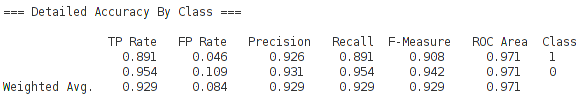
\includegraphics[width=\textwidth]{pictures/accuracy.png}
			\caption{\label{accuracy} Performances du modèle}
			\end{center}
			\end{figure}
			
			\begin{figure}[h]
			\begin{center}
			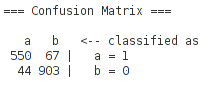
\includegraphics[]{pictures/confusion_matrix.png}
			\caption{\label{matrix} Matrice de confusion}
			\end{center}
			\end{figure}
			
		\end{homeworkSection}
			
		\begin{homeworkSection}{2.3}
			
			Donnez un exemple de contre-mesure de type Tokenization attack qu’un spammeur
			pourrait facilement utiliser afin de contourner un filtre basé uniquement sur la fréquence
			d’apparition de certains mots. Votre méthode ne doit pas modifier la signification du
			message et ne doit pas ajouter de nouveaux mots. Appliquez votre méthode au message
			suivant:\\

			\textit{DEAR RECEIVER,\\
			You have just received a Taliban virus. Since we are not so technologically
			advanced in Afghanistan, this is a MANUAL virus. Please click on
			this link (http://clickme.com) to delete all the files on your hard disk
			yourself and send this mail to everyone you know.
			Thank you very much for helping us.\\	\\
			-Taliban hacker.}\\

			\problemAnswer{
			
			}
					
		\end{homeworkSection}
		
			
	\end{homeworkProblem}